\subsection{Externe Merkmale des Gehirns}
\label{subsec:Externe_Merkmale}
%%%%%%%%%%%%%%%%%%%%%%%%%%%%%%%%%%%%%%%%%%%%%%%%%%%%%%%%%%%
%%%%%%%%%%%%%%%%%%%%%%%%%%%%%%%%%%%%%%%%%%%%%%%%%%%%%%%%%%%

\subsubsection{Hirnhäute} \index{Hirnhäute}
%%%%%%%%%%%%%%%%%%%%%%%%%%%%%%%%%%%%%%%%%%%%%%%%%%%%%%%%%%%

Drei Hirnhäute liegen zwischen dem Gehirn und dem Schädelknochen (Abb.~\ref{fig:hirnhaeute}). Die äußerste Schicht ist die \textbf{Dura mater}, auch harte Hirnhaut genannt. Sie ist lederartig, unelatisch und fest und umgibt schützend sowohl Gehirn als auch Rückenmark. Die spinnennetzartige \textbf{Arachnoidae mater encephali}, oder auch Spinnenhaut, befindet sich dirket unter der Dura mater. Die unterste Schicht bildet die \textbf{Pia mater}, auch weiche Hirnhaut genannt. Diese dünne Haut schmiegt sich eng an die Oberfläche des Gehirns an. Entlang der Pia mater verlaufen viele Blutgefäße, die schließlich ins darunterliegende Gehirn führen \textsuperscript{\cite[Kap.~7]{neurowissenschaften_baer}}. Zwischen der Arachnoidea und der Pia mater befindet sich der \textbf{Subarachnoidalraum}. Dieser ist mit Liquor cerebrospinalis\index{Liquor cerebrospinalis} gefüllt. In dieser dünnen Schicht aus farbloser Flüssigkeit schwimmt das Gehirn innerhalb des Schädels \textsuperscript{\cite[Kap.~7]{neurowissenschaften_baer}}.

\begin{figure}[H]
	\centering
	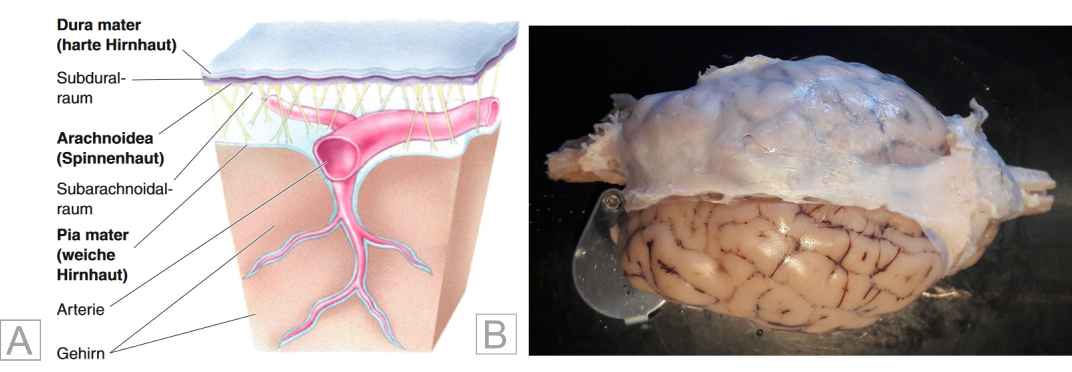
\includegraphics[width=\textwidth]{pictures/Bilder_Jule/Andere/hirnhaeute2.png}
	\caption[Die Hirnhäute]{\textbf{Die Hirnhäute.} \textbf{A}: Anordnung der drei Hirnhäute als Schema. \textbf{B}: Veranschaulichung der Hirnhäute am Schafhirn. Die  rostrale Seite ist nach links, die caudale nach rechts orientiert. Über der rechten Hemisphäre (oben) ist die Dura mater zu sehen. Auf der linken Hemisphäre (unten) ist die Pia mater zu sehen. Die Dura mater Arachnoidea wurde von dieser Hälfte inklusive Arachnoidea entfernt.\\
	Abbildung~A aus \textit{Neurowissenschaften}, Bear et al. \textsuperscript{\cite[Kap.~7]{neurowissenschaften_baer}}.}
	\label{fig:hirnhaeute}
\end{figure}


\subsubsection{Anhängende Strukturen}
\label{subsubsec:Hirnanhangsstrukturen}
%%%%%%%%%%%%%%%%%%%%%%%%%%%%%%%%%%%%%%%%%%%%%%%%%%%%%%%%%%%

\subsubsection*{Riechepithelium} \index{Riechepithel}
%%%%%%%%%%%%%%%%%%%%%%%%%%%%%%%%%%%%%%%%%%%%%%%%%%%%%%%%%%%%

Das Riechepithelium befindet sich außerhalb des Gehirns und ist am rostralen Ende mit diesem Verbunden. Es kleidet als Anteil der Nasenschleimhaut die obere Nasenmuschel und die gegenüberliegende Nasenscheidewand aus und überdeckt  ein  System aus Strömungskörpern (Abb.~\ref{fig:Riechepithel}). Das Riechepithel stellt die erste Station der Riechbahn dar. In diesem mehrschichtigen Sinnesepithel sind die chemorezeptiven Riechsinneszellen lokalisiert. Die axonalen Fortsätze dieser Zellen ziehen bis in die vordere Schädelgrube, wo sich der Bulbus olfactorius\index{Bulbus olfactorius} befindet. Bei Spezies mit gutem Riechvermögen nehmen Riechepithel und Bulbus olfactorius mehr Platz ein als bei Tieren, für deren Lebensweise der Riechsinn verhältnismäßig weniger relevant ist, wie beispielsweise bei Menschenaffen.

\begin{figure}[H]
    \centering
    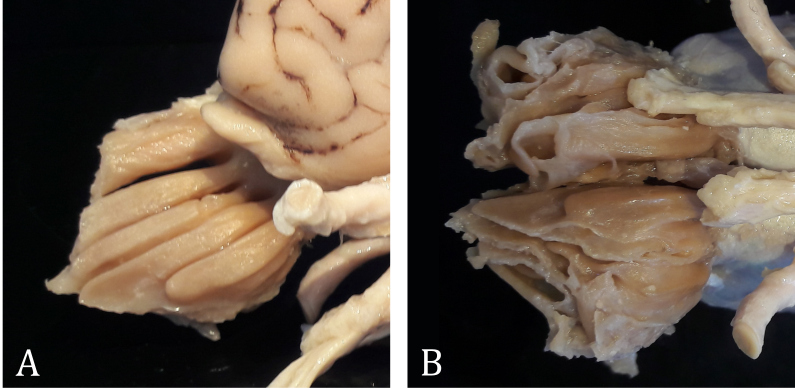
\includegraphics[width=0.8\textwidth]{pictures/Bilder_Jule/Schaf/Ausschnitte/Riechepithel.png}
    \caption[Riechepithelium Schaf]{\textbf{Riechepithelium Schaf}. Mediale (\textbf{A}) und inferiore (\textbf{B}) Ansicht des Riechepitheliums des Schafes.}
    \label{fig:Riechepithel}
\end{figure}{}


\subsubsection*{Hypophyse}
\label{subsubsec:hypophyse} \index{Hypophyse! allgemein}
%%%%%%%%%%%%%%%%%%%%%%%%%%%%%%%%%%%%%%%%%%%%%%%%%%%%%%%%%%%%

Die Hypophyse liegt inferior, leicht caudal des Chiamsa opticums und rostral des Mammillarkörpers. Über den Hypophysenstiel (Infundibulum) hängt sie am Hypothalamus (Abb.~\ref{fig:hypophyse}) \textsuperscript{\cite[Kap.~4]{trepel2011neuroanatomie}}. Die Hypophyse besteht aus zwei Teilgebieten, der Neurohypophyse\index{Hypophyse! Neurohypophyse} und der Adenohypophyse\index{Hypophyse! Adenohypophyse}. Dabei ist lediglich die \textbf{Neurohypophyse} (Hypophysenhinterlappen) Teil des Diencephalons. Die Neurohypophyse besitzt keine dichte Blut-Hirn-Schranke. Dadurch können Hormone, die von den dort lokalisierten Nervenzellen sezerniert werden, via Neurosekretion ins Blut gelangen. Die deutlich größere \textbf{Adenohypophyse} (Hypophysenvorderlappen) umhüllt teilweise den kleineren Hypophysenhinterlappen. Sie ist kein Bestandteil des Gehirns, sie ist lediglich an das Diencephalon angelagert. Somit besteht die Adenohypophyse nicht aus Nervengewebe, sondern aus Drüsenepithel. Durch die dort gebildeten glandotropen Hormone kann die Adenohypophyse auf endokrine Drüsen, wie die Schilddrüse oder die Nebennierenrinde, wirken. Diese Drüsen nehmen dann durch die Produktion eigener Hormone  Einfluss auf periphere Organe. Auch Effektorhormone werden in der Adenohypophyse gebildet. Diese können direkt, ohne Zwischenschaltung weiterer Drüsen, auf periphere Organe wirken. Die Hormone der Adenohypophyse sind unter anderem an der Pigmentierung der Haut, an der Milchbildung in der Brustdrüse, am Körperwachstum und an der Reifung von Ei- und Spermienzellen beteiligt. Generell ist die Hypophyse als das hormonelle 'Ausführungsorgan' des Hypothalamus\index{Hypothalamus} (Kap.~\ref{subsubsec:Hypothalamus}) zu betrachten  \textsuperscript{\cite[Kap.~8]{trepel2011neuroanatomie}}.

\begin{figure}[H]
    \centering
    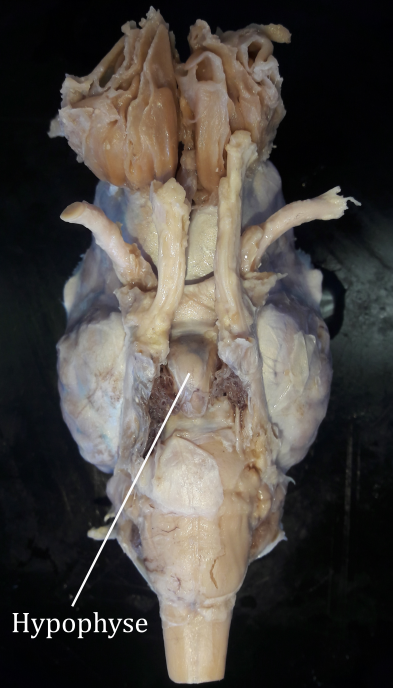
\includegraphics[width=0.5\textwidth]{pictures/Bilder_Jule/Schaf/Aussenansicht/Hypophyse.png}
    \caption[Hypophyse Schaf]{\textbf{Hypophyse Schaf}}
    \label{fig:hypophyse}
\end{figure}